% % % % % % % % % % % % % % % % % % % % % % % % % % % % % % % % % %
%\documentclass[runningheads]{llncs}
%\documentclass[10pt,letterpaper,twocolumn]{article}
\documentclass{sig-alternate}


% packages
\usepackage{xspace}
\usepackage{ifthen}
\usepackage{amsbsy}
\usepackage{amssymb}
\usepackage{balance}
\usepackage{booktabs}
\usepackage{graphicx}
\usepackage{multirow}
\usepackage{needspace}
\usepackage{microtype}
\usepackage{bold-extra}
\usepackage{subfigure}
\usepackage{wrapfig}


% constants
\newcommand{\Title}{Correlation Between Dependencies and Complexity: An Empirical Study}
\newcommand{\TitleShort}{\Title}
\newcommand{\Authors}{Santiago Vidal, Alexandre Bergel, Claudia Marcos}
\newcommand{\AuthorsShort}{S. Vidal, A. Bergel, C. Marcos}

% references
\usepackage[colorlinks]{hyperref}
\usepackage[all]{hypcap}
\setcounter{tocdepth}{2}
\hypersetup{
	colorlinks=true,
	urlcolor=black,
	linkcolor=black,
	citecolor=black,
	plainpages=false,
	bookmarksopen=true,
	pdfauthor={\Authors},
	pdftitle={\Title}}

\def\chapterautorefname{Chapter}
\def\appendixautorefname{Appendix}
\def\sectionautorefname{Section}
\def\subsectionautorefname{Section}
\def\figureautorefname{Figure}
\def\tableautorefname{Table}
\def\listingautorefname{Listing}

% source code
\usepackage{xcolor}
\usepackage{textcomp}
\usepackage{listings}
\definecolor{source}{gray}{0.9}
\lstset{
	language={},
	% characters
	tabsize=3,
	upquote=true,
	escapechar={!},
	keepspaces=true,
	breaklines=true,
	alsoletter={\#:},
	breakautoindent=true,
	columns=fullflexible,
	showstringspaces=false,
	basicstyle=\footnotesize\sffamily,
	% background
	frame=single,
    framerule=0pt,
	backgroundcolor=\color{source},
	% numbering
	numbersep=5pt,
	numberstyle=\tiny,
	numberfirstline=true,
	% captioning
	captionpos=b,
	% formatting (html)
	moredelim=[is][\textbf]{<b>}{</b>},
	moredelim=[is][\textit]{<i>}{</i>},
	moredelim=[is][\color{red}\uwave]{<u>}{</u>},
	moredelim=[is][\color{red}\sout]{<del>}{</del>},
	moredelim=[is][\color{blue}\underline]{<ins>}{</ins>}}
\newcommand{\ct}{\lstinline[backgroundcolor=\color{white},basicstyle=\footnotesize\ttfamily]}
\newcommand{\lct}[1]{{\small\tt #1}}

% tikz
% \usepackage{tikz}
% \usetikzlibrary{matrix}
% \usetikzlibrary{arrows}
% \usetikzlibrary{external}
% \usetikzlibrary{positioning}
% \usetikzlibrary{shapes.multipart}
% 
% \tikzset{
% 	every picture/.style={semithick},
% 	every text node part/.style={align=center}}

% proof-reading
\usepackage{xcolor}
\usepackage[normalem]{ulem}
\newcommand{\ra}{$\rightarrow$}
\newcommand{\ugh}[1]{\textcolor{red}{\uwave{#1}}} % please rephrase
\newcommand{\ins}[1]{\textcolor{blue}{\uline{#1}}} % please insert
\newcommand{\del}[1]{\textcolor{red}{\sout{#1}}} % please delete
\newcommand{\chg}[2]{\textcolor{red}{\sout{#1}}{\ra}\textcolor{blue}{\uline{#2}}} % please change
\newcommand{\chk}[1]{\textcolor{ForestGreen}{#1}} % changed, please check

% comments \nb{label}{color}{text}
\newboolean{showcomments}
\setboolean{showcomments}{true}
\ifthenelse{\boolean{showcomments}}
	{\newcommand{\nb}[3]{
		{\colorbox{#2}{\bfseries\sffamily\scriptsize\textcolor{white}{#1}}}
		{\textcolor{#2}{\sf\small$\blacktriangleright$\textit{#3}$\blacktriangleleft$}}}
	 \newcommand{\version}{\emph{\scriptsize$-$Id$-$}}}
	{\newcommand{\nb}[2]{}
	 \newcommand{\version}{}}
\newcommand{\rev}[2]{\nb{Reviewer #1}{red}{#2}}
\newcommand{\ab}[1]{\nb{Alexandre}{blue}{#1}}
\newcommand{\vp}[1]{\nb{Vanessa}{orange}{#1}}

% graphics: \fig{position}{percentage-width}{filename}{caption}
\DeclareGraphicsExtensions{.png,.jpg,.pdf,.eps,.gif}
\graphicspath{{figures/}}
\newcommand{\fig}[4]{
	\begin{figure}[#1]
		\centering
		\includegraphics[width=#2\textwidth]{#3}
		\caption{\label{fig:#3}#4}
	\end{figure}}

\newcommand{\largefig}[4]{
	\begin{figure*}[#1]
		\centering
		\includegraphics[width=#2\textwidth]{#3}
		\caption{\label{fig:#3}#4}
	\end{figure*}}
	
\newcommand{\wrapfig}[5]{	
\begin{wrapfigure}{#1}{#2\textwidth}
  \begin{center}
    \includegraphics[width=#3\textwidth]{#4}
  \end{center}
  \caption{\label{fig:#4}#5}
\end{wrapfigure}}

% abbreviations
\newcommand{\ie}{\emph{i.e.,}\xspace}
\newcommand{\eg}{\emph{e.g.,}\xspace}
\newcommand{\etc}{\emph{etc.}\xspace}
\newcommand{\etal}{\emph{et al.}\xspace}

% lists
\newenvironment{bullets}[0]
	{\begin{itemize}}
	{\end{itemize}}

\newcommand{\seclabel}[1]{\label{sec:#1}}
\newcommand{\secref}[1]{Section~\ref{sec:#1}}
\newcommand{\appref}[1]{Appendix~\ref{sec:#1}}
\newcommand{\figlabel}[1]{\label{fig:#1}}
\newcommand{\figref}[1]{Figure~\ref{fig:#1}}
\newcommand{\tablabel}[1]{\label{tag:#1}}
\newcommand{\tabref}[1]{Table~\ref{fig:#1}}


%Specialized macros
\pagenumbering{arabic}

\begin{document}

\title{\Title}
%\titlerunning{\TitleShort}

\author{\Authors\\[3mm]
Department of Computer Science (DCC)\\ University of Chile, Santiago, Chile\\[1 ex]
} 
%\authorrunning{\AuthorsShort}

\maketitle

%\emph{This paper makes use of colored figures. Though colors are not mandatory for full understanding, we recommend  the use of a colored printout.}

\begin{abstract}
%	What's the problem.
The amount of external dependencies is commonly considered as a source of complexity.  More a component has external dependencies, more complex it becomes. However, this has never been empirically verified. In addition, it is not clear which kind of dependencies is more related to the complexity.
%	Why is the problem a problem?


%	What's the surprising idea?

We empirically show that the complexity metrics of a software element are strongly correlated with the external dependencies the element has.

%	What's the consequence?
We are able to simplify X software by decreasing the dependencies.

\end{abstract}

%: % % % % % % % % % % % % % % % % % % % % % % % % % % % % % % % % %
\section{Introduction}\seclabel{introduction}

The quality of a software source code is usually perceived as the cost to change it~\cite{}.

Software dependencies is often considered as a primary source of complexity. More a component has dependencies on its executing environment or other components, more complex the component is~\cite{Sang05a}. 

Relating some metrics to some quality attributes has received attention from the community.

Briand \etal~\cite{Bria00a} investigated the relationship between design measurements in object-oriented systems and the overall quality of the developed software. The quality is measured by fault-proneness. 

Relation between design metrics and productivity or effort ~\cite{Chida98a}

Relation between design metrics and the amount of maintenance modifications(?)~\cite{Li93a}




~\cite{Baxt06a}

~\cite{Taub11a}


The research questions addressed in this paper are:
\begin{itemize}
\item[A -] \emph{How closely the number of external dependencies is related to the code complexity?}
\item[B -] \emph{Can the number of external dependencies be used as a proxy for measuring the code complexity?}
%\item[C -] \emph{Can the complexity system be reduced by reducing the dependencies?}
\end{itemize}

We provide a number of contributions based on a large empirical study:
\begin{itemize}
\item complexity metrics are strongly correlated with dependencies: more complex a class is, more dependencies to other classes the class has
\end{itemize}


%: % % % % % % % % % % % % % % % % % % % % % % % % % % % % % % % % %
\section{Methodology}\seclabel{methodology}

Our methodology is summarized as follows:

\begin{enumerate}
\item Choose a list of relevant software programs. From squeaksource.com
\item Process each version of these programs in the Moose software analysis platform. 
\item Establish the correlation between each metric and the statistical moment for each dependency relation we considered.
\item Identify the minimum amount of kind of dependencies to have a maximum fit to a predictive models.
%\item Reduce the amount of dependencies for a representative portion of source code by means of manual refactorings.
%\item Measure the evolution of the complexity metrics
\end{enumerate}

%=========
\subsection{Project Repositories}

The list of projects and their size is given in \appref{listOfSoftware}
From squeaksource.com


%=========
\subsection{Process each program version}

Thanks to its language independent metamodel, Moose is able to analyzes software

The complete software source code is an instance of the metamodel.

Run the complexity metrics for each version.


%=========
\subsection{Power-law?}

\ab{Check if we have to talk about this. Probably yes}


%=========
\subsection{Correlation between metrics and statistical moment}



%: % % % % % % % % % % % % % % % % % % % % % % % % % % % % % % % % %
\section{Correlation between code complexity and dependencies}






%=========
\subsection{Code complexity}
There is a large number of metrics to measure the source code complexity.
The complexity metrics traditionally found are: LOC, Cyclomatic Complexity (1 \& 2 \& 3), NOM ...

McCabe's Cyclomatic Complexity (MCC)~\cite{McCa76a} counts branching and control flow in a program.
Halstead's complexity metric measure the number of unique operators and operands. 


To check: \url{http://yunus.hacettepe.edu.tr/~sencer/complexity.html}


The correlation is calculated to different granularity elements (methods, classes, and packages) using complexity and dependence metrics. The metrics used in order to determine the complexity of a system are:
\begin{itemize}%Contar para cada uno que se calcula para metodos, clases y paquetes
\item Cyclomatic complexity: The cyclomatic complexity of a method is the number of decision points in the control flow graph of the method. The decision points are declarations such as if, for, while, try/catch, etc. The number of decision points in a statement can vary depending, for example, the complexity of Boolean expressions. As this metric is calculate to a method, in order to calculate the complexity of a class we sum the cyclomatic complexity of all the methods of the class. A similar approach is followed to calculate the complexity of a package. 
\item Lines of code: the total number of lines of codes is an indicator to measure how complex a system is. In this case we measure the lines of codes of a method, a class, or a package (i.e. the sum of the lines of code of the classes that it contains).
\item Number of invocations: other metrics that are helpful to determine the complexity of a system are fan-in and fan-out. The complexity metric is calculated as: Length x (Fan-in x Fan-out)$^{2}$ where length is a metric such as lines of code or cyclomatic complexity. In the case of the classes and the packages the fan-in and fan-out metrics are calculated as incoming and outgoing invocations respectively.
\end{itemize}
%=========
\subsection{Source code element dependencies}

Between methods, classes and packages (namespaces)

In order to calculate the dependencies of an entity (method, class or package) several strategies can be followed:
\begin{itemize}
\item Outgoing invocations (OI): this kind of invocation computes all the packages, classes and methods referenced by an entity. 
\item All dependencies (AD): this kind of invocation comprises the outgoing invocations and add the static dependences such as accesses, references and inheritances.
\end{itemize}
An important consideration is that during the calculation of these metrics those dependencies that loop back to its receiver can be avoided. In this way we can filter only those dependencies with other entities (methods, classes or packages).

Also, the dependencies of an entity can be refined according the scope of them. Specifically, we use scope for methods, classes and packages. For example, if the outgoing invocations of the class \emph{A} are calculated and refined using the package scope the dependencies obtained will be packages which contain classes referenced by the class \emph{A}.

%poner un pequeño ejemplo para mostrar las diferencias entre los distintos tipos de dependencias

\begin{table*}
\begin{tabular}{|c|c|c|c|c|}
\hline 
 & LOC & CC & FanInFanOut/LOC & FanInFanOut/CC\tabularnewline
\hline 
\hline 
All dependencies  & 0.68 & 0.91 & 0.70 & 0.60\tabularnewline
\hline 
All dependencies (WL) & 0 & 0 & 0 & 0\tabularnewline
\hline 
Outgoing invocations & 0.67 & 0.85 & 0.72 & 0.71\tabularnewline
\hline 
Outgoing invocations (WL) & 0.67 & 0.85 & 0.71 & 0.71\tabularnewline
\hline 
All dependencies (ACS) & 0.006 & 0.50 & 0.30 & 0.34\tabularnewline
\hline 
All dependencies (ACS WL) & 0 & 0 & 0 & 0\tabularnewline
\hline 
Outgoing invocations (ACS) & 0.005 & 0.48 & 0.35 & 0.40\tabularnewline
\hline 
Outgoing invocations (ACS WL) & 0.02 & 0.61 & 0.34 & 0.40\tabularnewline
\hline 
All dependencies (APS) & 0.27 & 0.90 & 0.35 & 0.41\tabularnewline
\hline 
All dependencies (APS WL) & 0 & 0 & 0 & 0\tabularnewline
\hline 
Outgoing invocations (APS) & 0.25 & 0.90 & 0.34 & 0.40\tabularnewline
\hline 
Outgoing invocations (APS WL) & 0.32 & 0.90 & 0.35 & 0.41\tabularnewline
\hline 
All dependencies (ANS) & -0.33 & 1 & -0.5 & 2,78E-01\tabularnewline
\hline 
All dependencies (ANS WL) & 0 & 0 & 0 & 0\tabularnewline
\hline 
Outgoing invocations (ANS) & 0 & 0 & 0 & 0\tabularnewline
\hline 
Outgoing invocations (ANS WL) & 0 & 0 & 0 & 0\tabularnewline
\hline 
\end{tabular}

\medskip{}
WL= without loops; ACS= at class scope; APS= at package scope; ANS= at namespace scope
\caption{Methods results}



\end{table*}

%=========
\subsection{Correlation}

\begin{tabular}{|c|c|c|c|}\hline
dep - metric  & LOC & McCabe & Halstead\\\hline
m$<->$m	&	& & \\\hline
c$<->$c	&	& & \\\hline
p$<->$p	&	& & \\\hline
m$<->$c	&	& & \\\hline
m$<->$p	&	& & \\\hline
c$<->$m	&	& & \\\hline
c$<->$p	&	& & \\\hline
p$<->$m	&	& & \\\hline
p$<->$c	&	& & \\\hline
\end{tabular}


Four case studies were conducted in which several version of Java an Smalltalk systems were analyzed. Specifically, we analyze Mondrian\footnote{\url{http://www.moosetechnology.org/tools/mondrian}}, Versionner\footnote{\url{http://www.squeaksource.com/Versionner}}, Vuze\footnote{\url{http://www.vuze.com/}}, and JFreeChart\footnote{\url{www.jfree.org/jfreechart}}. For each version of these systems several metrics of complexity and dependence were calculated as mentioned above. Both kind of measurements were calculated for packages, classes, and methods. For each one of these measurements the results of all the versions of a system were study conducting a regression analysis.

After conducting the case studies we found evidence of the existence of a correlation between dependencies and complexity measurements.
Regarding the classes, a strong correlation was found between AD and LOC, AD and WMC, OI and LOC, and OI and WMC (\figref{Correlation-comparison}). The fact that no correlation was identified when the dependencies are calculated only to a subset of entities (such as at class scope or at package scope), indicates that the changes in the dependences that affect the complexity of a system are global instead of local. That is, if there is the complexity is  increased that is because of an increment of all the dependencies.
Similar results were obtained for packages and methods. In the case of packages interesting correlations were found between AD and LOC, AD and CC, OI and LOC, and OI and CC. In regard to the methods, the correlations were found between  AD and LOC, and OI and LOC. 



\begin{figure*}
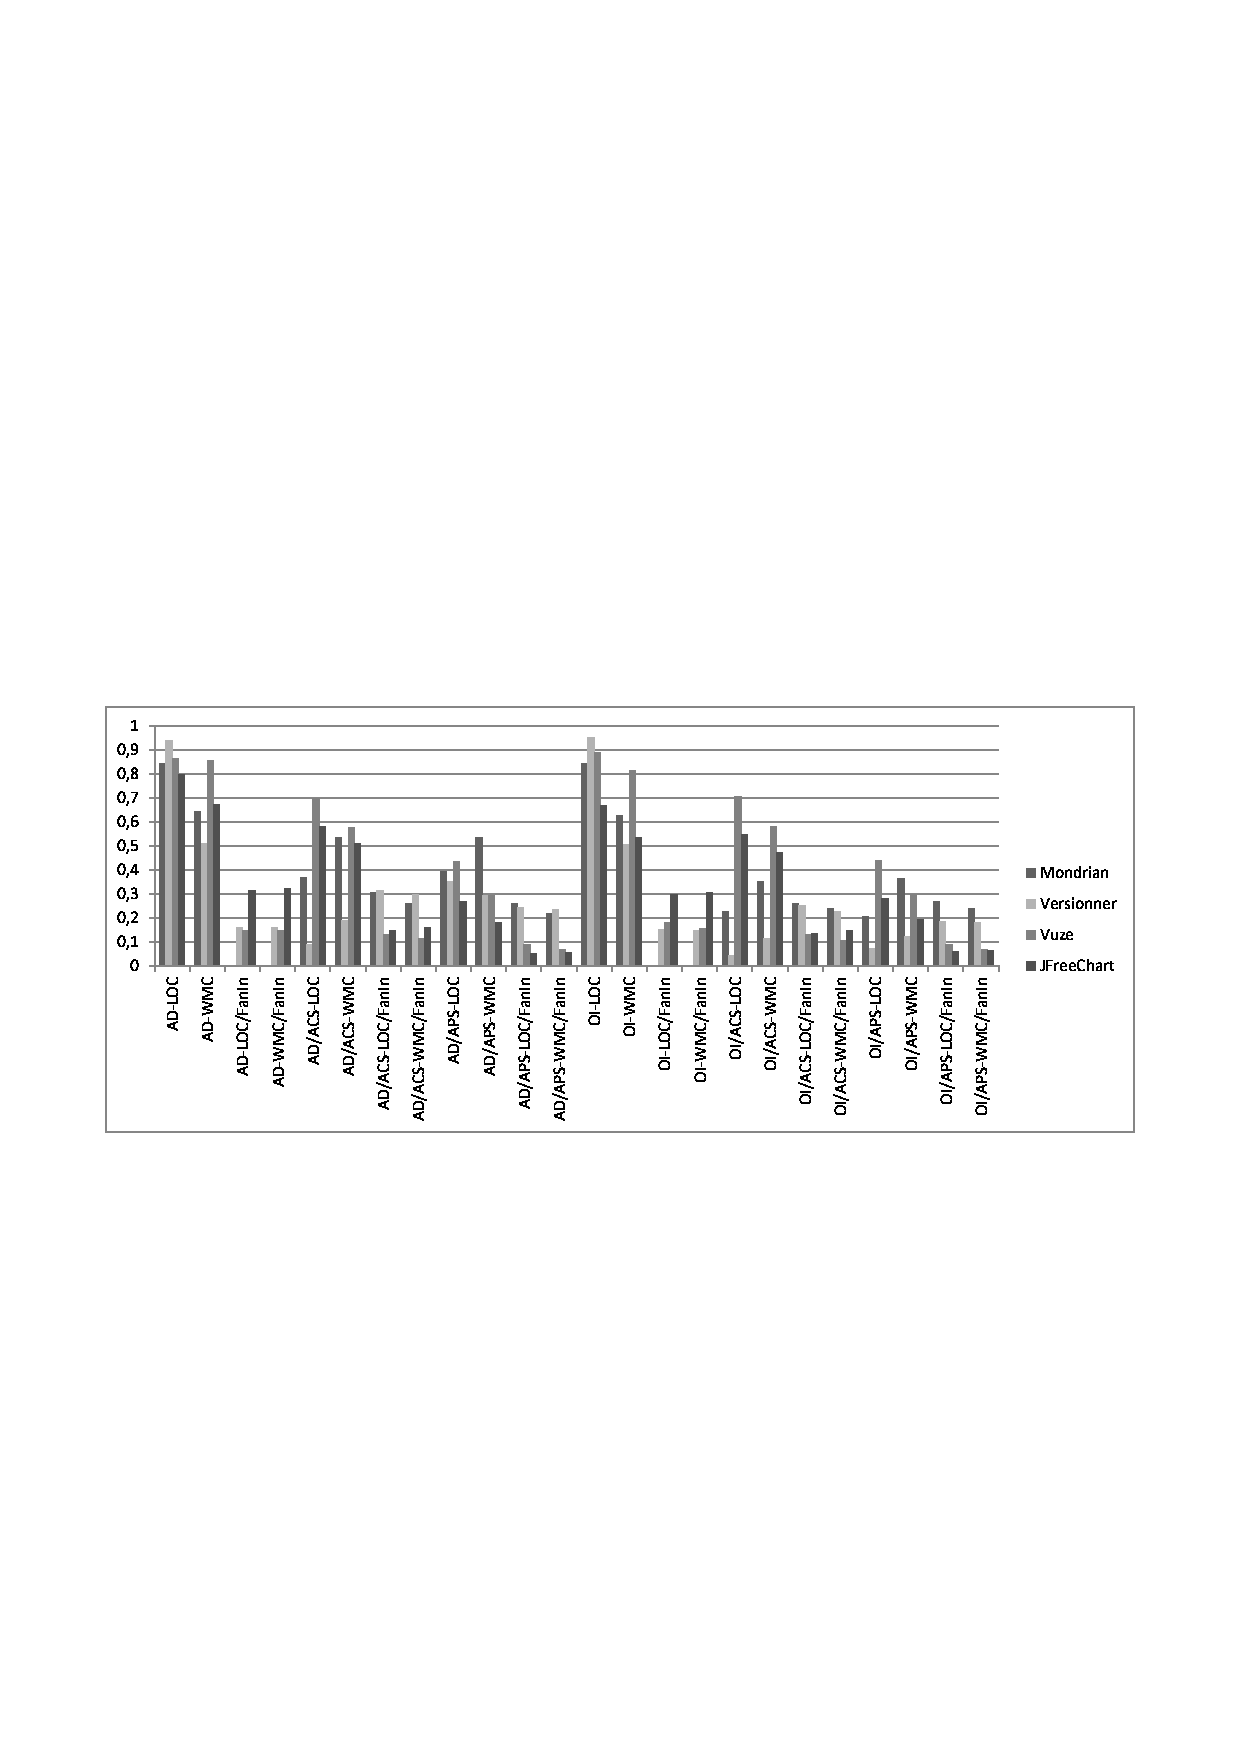
\includegraphics[bb=52bp 300bp 540bp 500bp,clip]{ClassesMetricsComparison}

\caption{Correlation comparison for classes measurements.\figlabel{Correlation-comparison}}


\end{figure*}




%: % % % % % % % % % % % % % % % % % % % % % % % % % % % % % % % % %
\section{Related Work}

Abram Hindle \etal~\cite{Hind08a} have shown that the code indentation is a reliable proxy for measuring the cyclomatic complexity

Dependency Structural Matrix~\cite{Sang05a}

%: % % % % % % % % % % % % % % % % % % % % % % % % % % % % % % % % %
\section{Conclusion}\seclabel{conclusion}

%\paragraph{Acknowledments} We thanks 

% % % % % % % % % % % % % % % % % % % % % % % % % % % % % % % % % %


%{\small
\bibliographystyle{plain}
\bibliography{scg}
%}

%: % % % % % % % % % % % % % % % % % % % % % % % % % % % % % % % % %
\appendix

\section{Analyzed software} \seclabel{listOfSoftware}

\begin{table}
\begin{tabular}{|l|l|l|}\hline
\textbf{name} & \textbf{language} & \textbf{LOC}\\
Mondrian\\
HealthReportProducer\\
Spy\\
Roassal\\
Versionner\\
Merlin\\
Tode\\
\end{tabular}
\caption{List of analyzed software}
\end{table}

\end{document}
